\section{REST-for-Physics libraries}

\label{sec:libraries}
% We define the different libraries in REST with a short description. We dedicate a section to the detector library since it is a central library that connects raw, geant4, and track libraries. And since REST was born to be used in the domain of rare event physics we always need a detector, but we are not forced to use it.

The main framework contains common tools required for centralized data access, visualization, and basic analysis routines, including generic REST-for-Physics \emph{metadata} classes and \emph{processes} that do not require \emph{event} specialization, i.e. they only need to access information at the \emph{analysis tree} level. More specialized routines, requiring a dedicated \emph{event} data type, such as time signal processing or detector event reconstruction, are organized into libraries; all classes belonging to the library keep a closer relation and therefore enhanced connectivity.

A library is usually associated only with one or two \emph{specific event} types, increasing the connectivity between different \emph{specific event processes} inside the same library. In this way, any combination of processes belonging to a particular library can be connected inside a data processing chain within its library domain. A dedicated library, the \emph{connectors} library, hosts those \emph{specific event processes} or \emph{specific metadata} objects that need to interconnect different libraries, keeping all inter-library dependencies bound together into a single entity and allowing each library to be fully operational in stand-alone mode.

A class belonging to a particular library will have its library name as a prefix at the class name. Therefore, the \emph{TRest} naming convention is extended in the case of the libraries to \emph{TRestLibName}, enabling the prompt identification of the library an object belongs to \footnote{In this context, we will continue highlighting the words that make reference to C++ objects using that pattern, such as \emph{TRestDetectorReadout} being written as \emph{detector readout}, or even omitting the library keyword, writing, for example, \emph{TRestDetectorGas} simply as \emph{gas}.}.

Even though new libraries might be added in the future to the framework, this section briefly describes those fundamental libraries that gave REST-for-Physics enough functionality and versatility to be used in different aspects of rare event searches experiments.

\subsection{The detector library}

The detector library\,\cite{REST_Detector_Git} has been designed to be used for event reconstruction inside a Time Projection Chamber (TPC) filled with a gaseous medium\footnote{The currrent version of REST-for-Physics has only been exploited with gaseous TPCs. However, a liquid TPC or even other detector technologies will probably share common detection elements, like the generic \emph{detector readout} implementation, or several detector physics processes. }. This library contains metadata class definitions that allow to describe the detector configuration: these can be \emph{drift volume} description, the \emph{detector readout} topology, the particular \emph{gas} properties (extracted using the Magboltz interface implemented by Garfield++) or others. It also integrates processes implementing routines for event reconstruction from real detector data and/or emulation of different physical response effects, e.g. including \emph{electron diffusion}, or artificially introducing the detector energy resolution by means of a \emph{smearing} process.

The \emph{readout} construction (see Figure\,\ref{fig:readouts}) is a crucial element of the detector library. This element permits the definition of an arbitrary number of \emph{readout planes}, containing an arbitrary number of \emph{readout modules}, composed of physical \emph{readout channels} that identify unambiguously with the acquisition channels of an electronics setup. The \emph{readout channels} are at the same time built with \emph{readout pixels}, the most basic element of a \emph{detector readout}. Such scheme allows to create any arbitrary and complex topology, with the capability to efficiently translate - back and forward - physical coordinates and electronic channels for readouts containing a few millions of pixels.

\begin{figure}[htb!]
  \centering
  \raisebox{-0.5\height}{
  \begin{tabular}{ccc}
  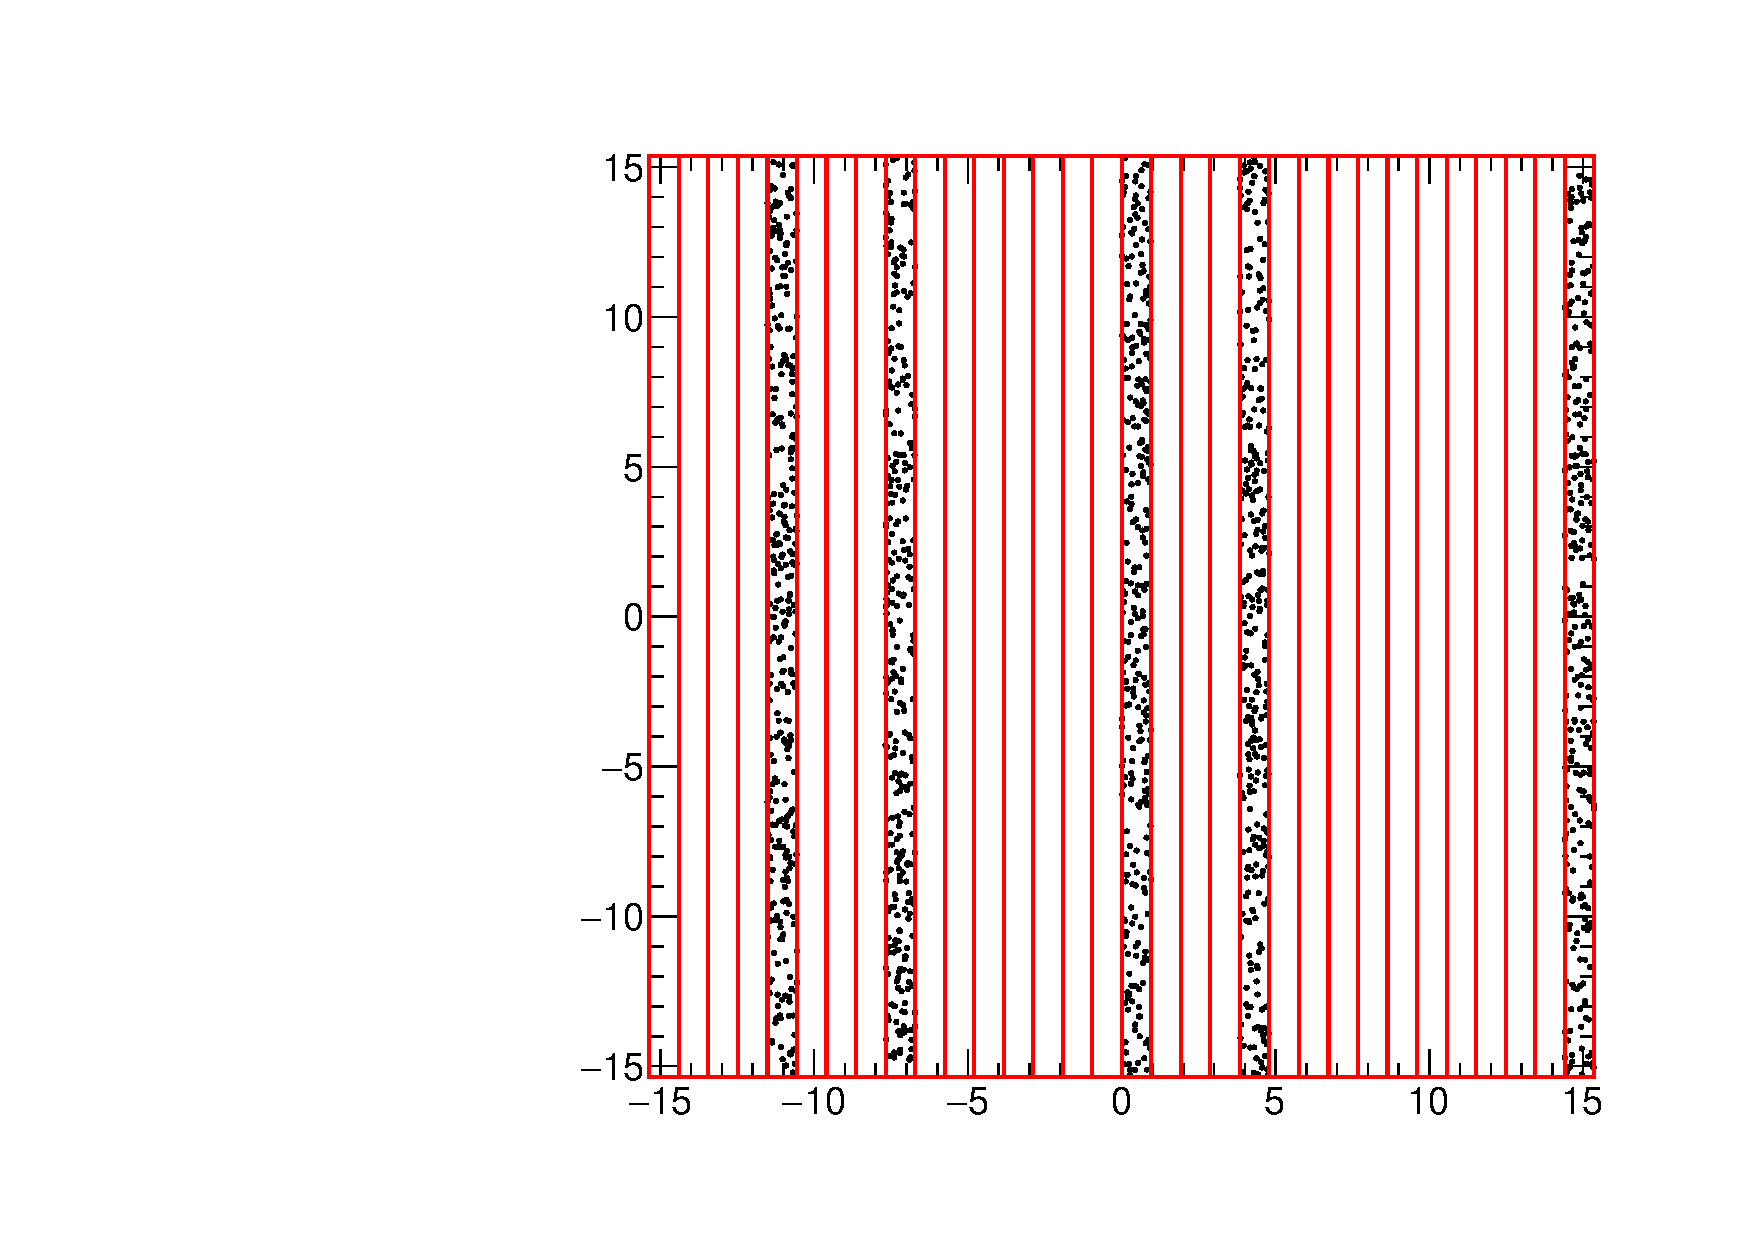
\includegraphics[width=0.3\textwidth]{images/stripped.pdf} & 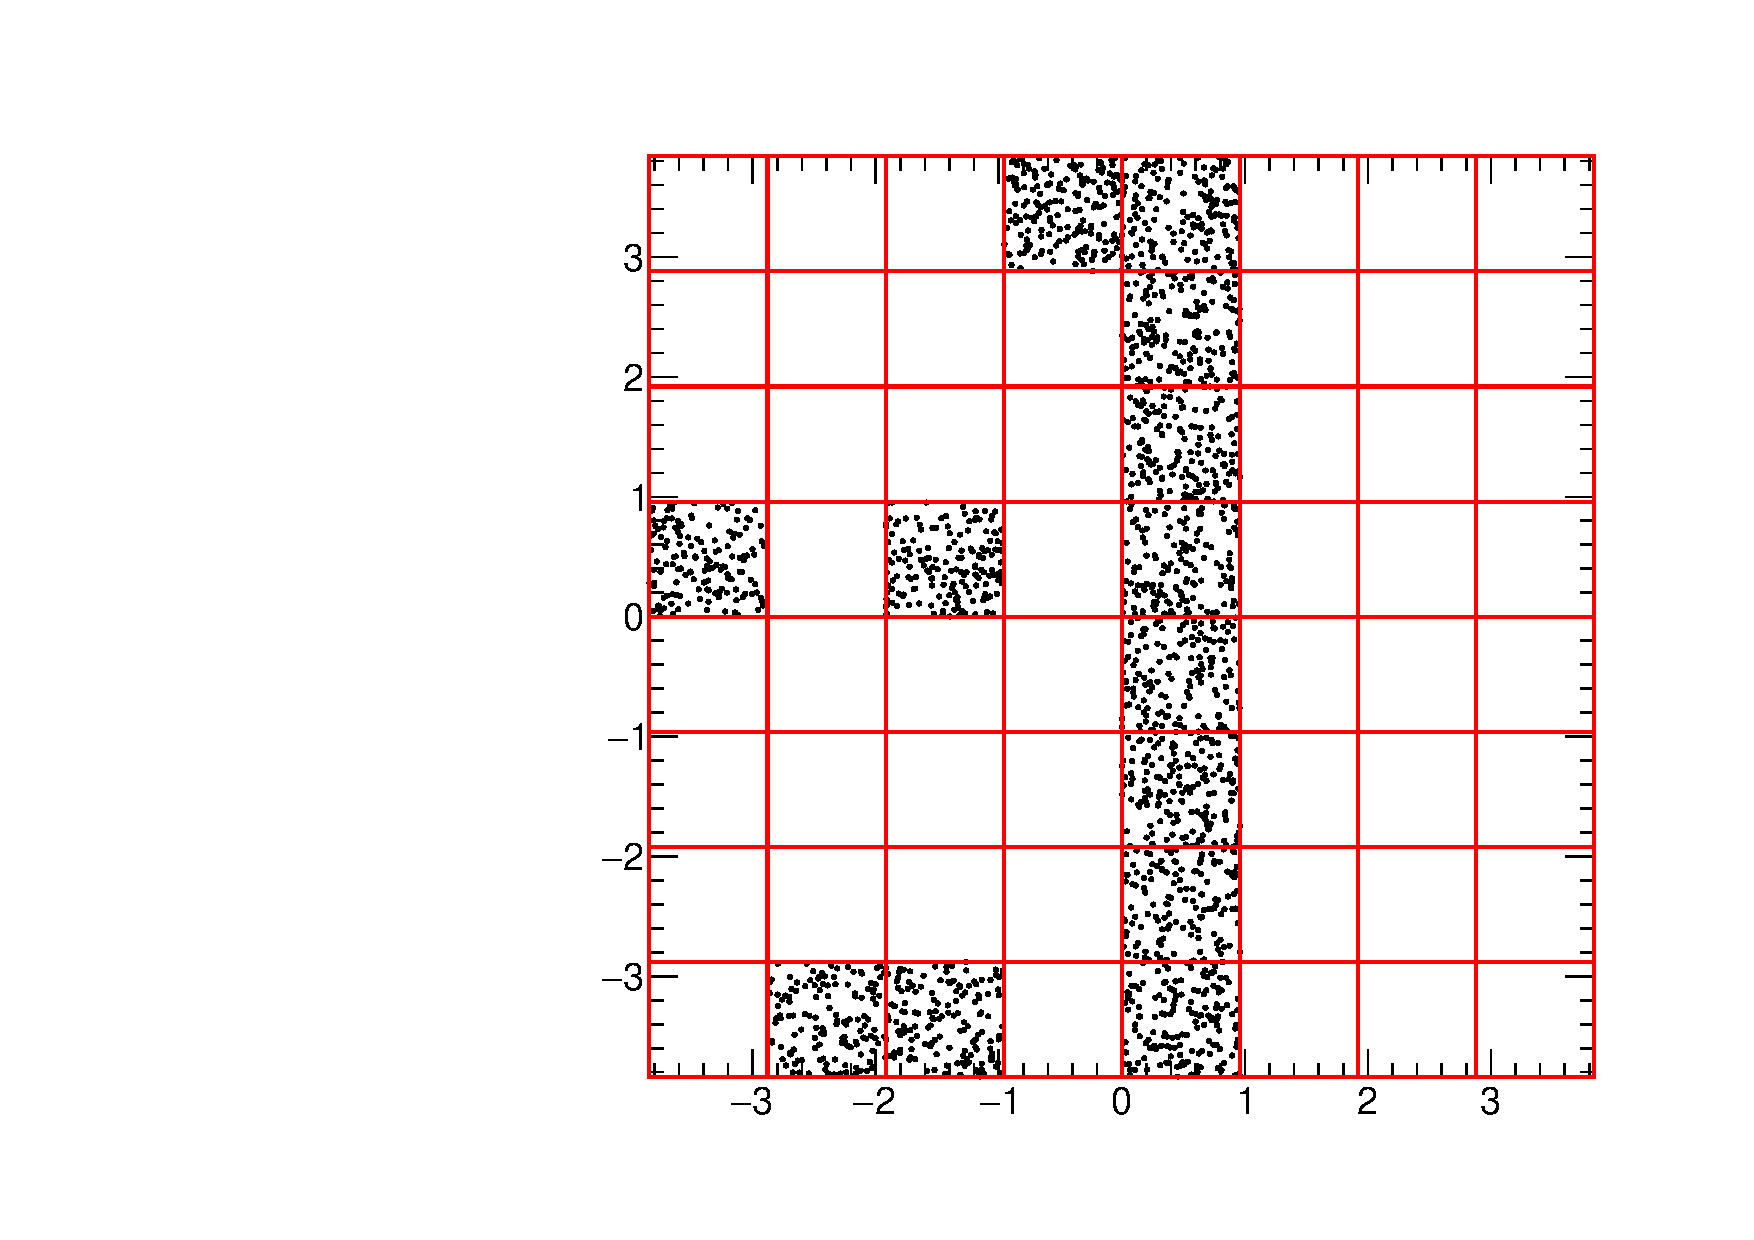
\includegraphics[width=0.3\textwidth]{images/pixel.pdf} & 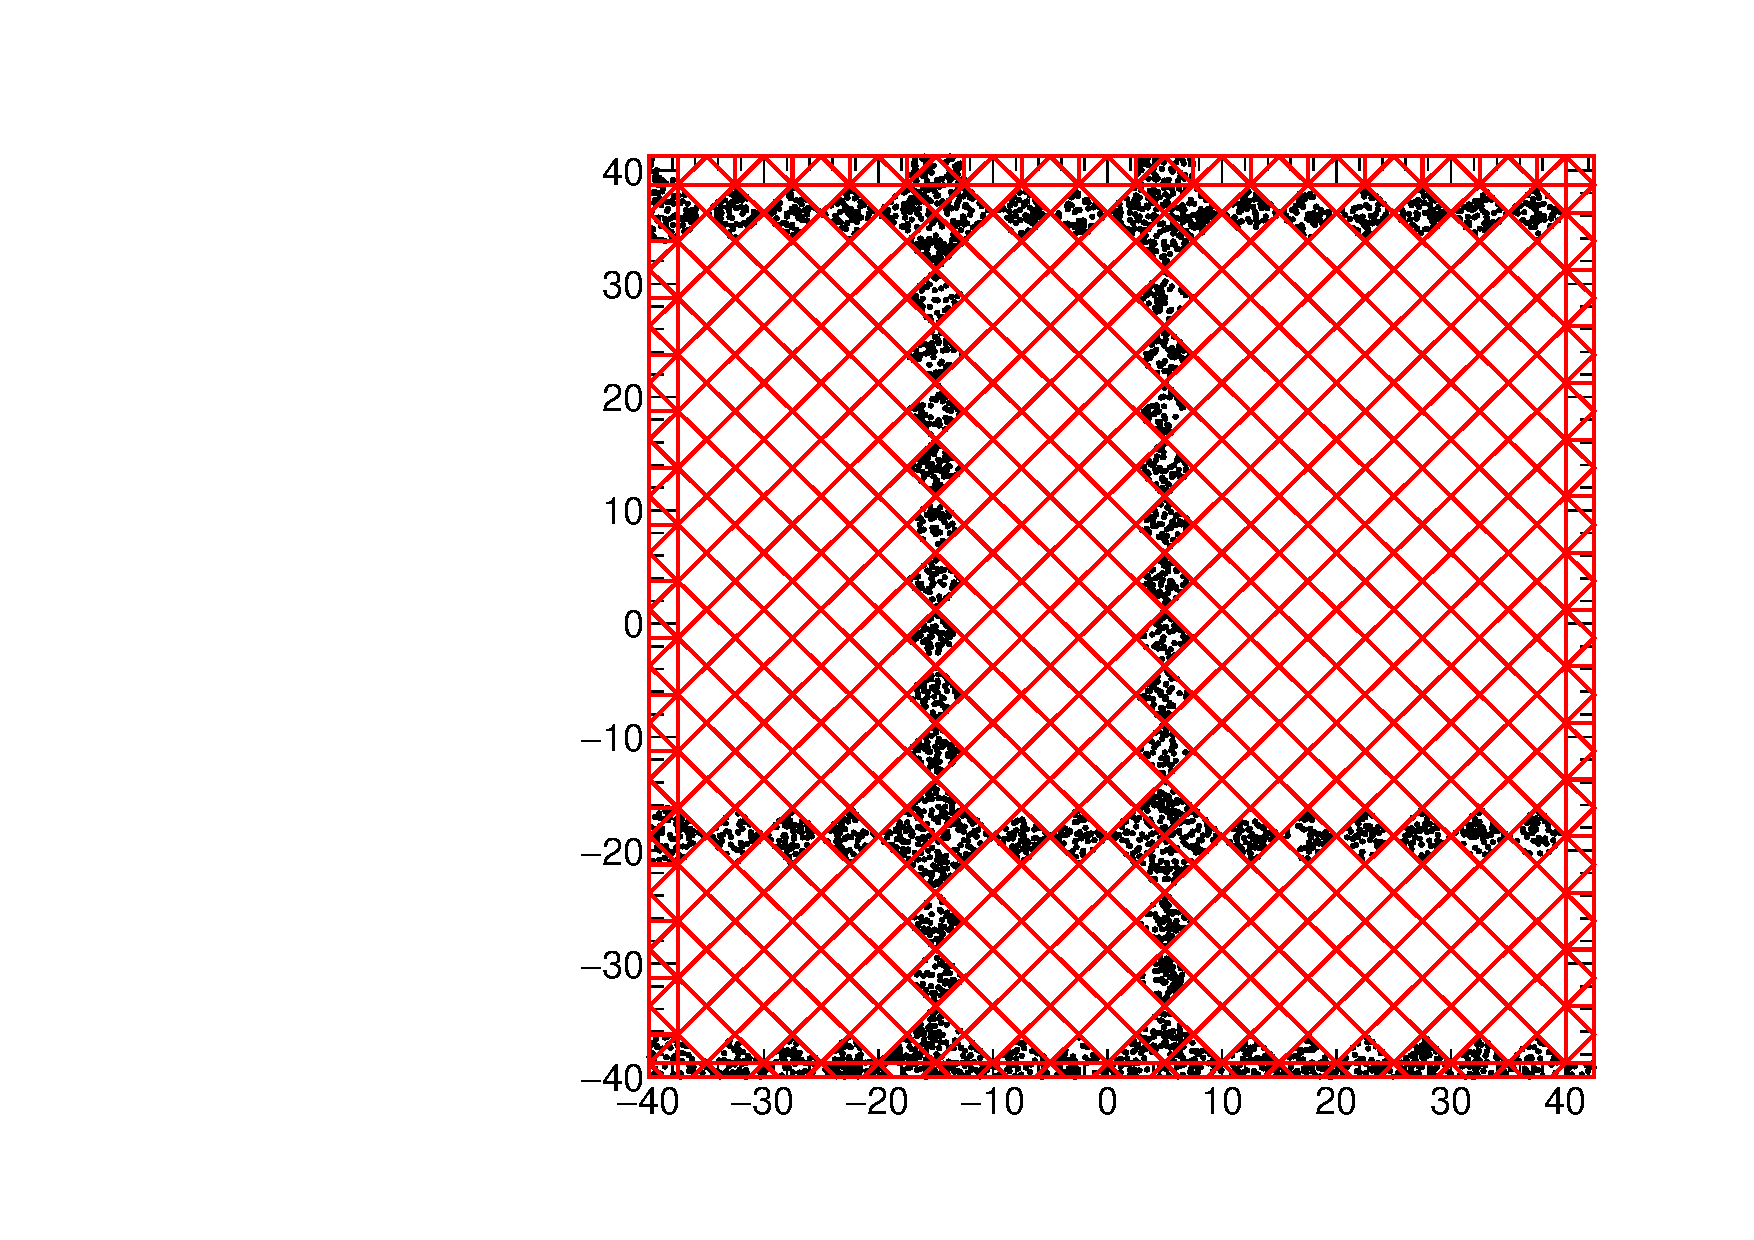
\includegraphics[width=0.3\textwidth]{images/microbulk.pdf} \\
  (a) & (b) & (c) \\
  \end{tabular}}
	\caption{Basic readout topologies that can be found at the \emph{basic-readouts} repository in REST-for-Physics. (a) A stripped \emph{readout channel} layout. (b) A pixel layout. (c) A more complex layout, where each \emph{channel} is composed of a few interconnected \emph{readout pixels} that create a stripped pattern. The red lines represent the boundaries of the \emph{readout pixels}, while the black dots are produced randomly by Monte Carlo. In our validation routines we enable only a few of the \emph{channels} to test the good behavior of the \emph{detector readout} implementation.}\label{fig:readouts}
\end{figure}

As any other library, the detector library provides an event type to encapsulate the detector data. Currently, and for convenience, it is the only library that defines two event types. The \emph{detector hits event} type, and the \emph{detector signal event} type. The \emph{hits event} defines a physical quantity, the energy deposits at the detector physical volume, using a 3-dimensional spatial coordinate representation. The \emph{signal event} describes the energy deposits as a function of the arrival time to the \emph{readout plane} associated to each detector electronics channel. The \emph{readout} implementation works as a dictionary between those two types; it is used to translate one event type into another by projecting the energy deposits into the \emph{readout channels}, or by recovering back the physical coordinate description from the readout channels information.

This library plays a central role in the description of the detector response and thus naturally includes connections to REST libraries related to raw electronics data processing (section\,\ref{sc:rawlib}), particle physics Monte Carlo event processing (section\,\ref{sc:geant4lib}) or physical track identification and pattern recognition routines (section\,\ref{sc:tracklib}). The processes responsible for such library inter-connectivity are hosted at an independent library, the connectors library (see section\,\ref{sc:connectorslib}).

\subsection{The raw library}\label{sc:rawlib}

The raw library\,\cite{REST_Raw_Git} implements a \emph{raw signal event} type that is suited to describe the time evolution of physical quantities that have been acquired with a fixed sampling rate. Inside this event type we may find an arbitrary number of \emph{raw signals} that, in our case, are identified with the induced currents at the electronic channels of our detector. Each \emph{raw signal} inside event definition contains usually the same number of samples, a value which is fixed during the \emph{raw signal} initialization. The data depth of the physical quantity described inside the \emph{raw signal} is 16-bits precision, which is enough to fit the typical values of electronic acquisition systems.

This library includes processes related to signal conditioning, such as signal shaping, de-convolution, pulse fitting, de-noising, Fast Fourier Transform operations, common noise reduction and other time-signal manipulation routines (see Figure\,\ref{fig:rawlib}). 

\begin{figure}[htb!]
  \centering
  \raisebox{-0.5\height}{
  \begin{tabular}{cc}
  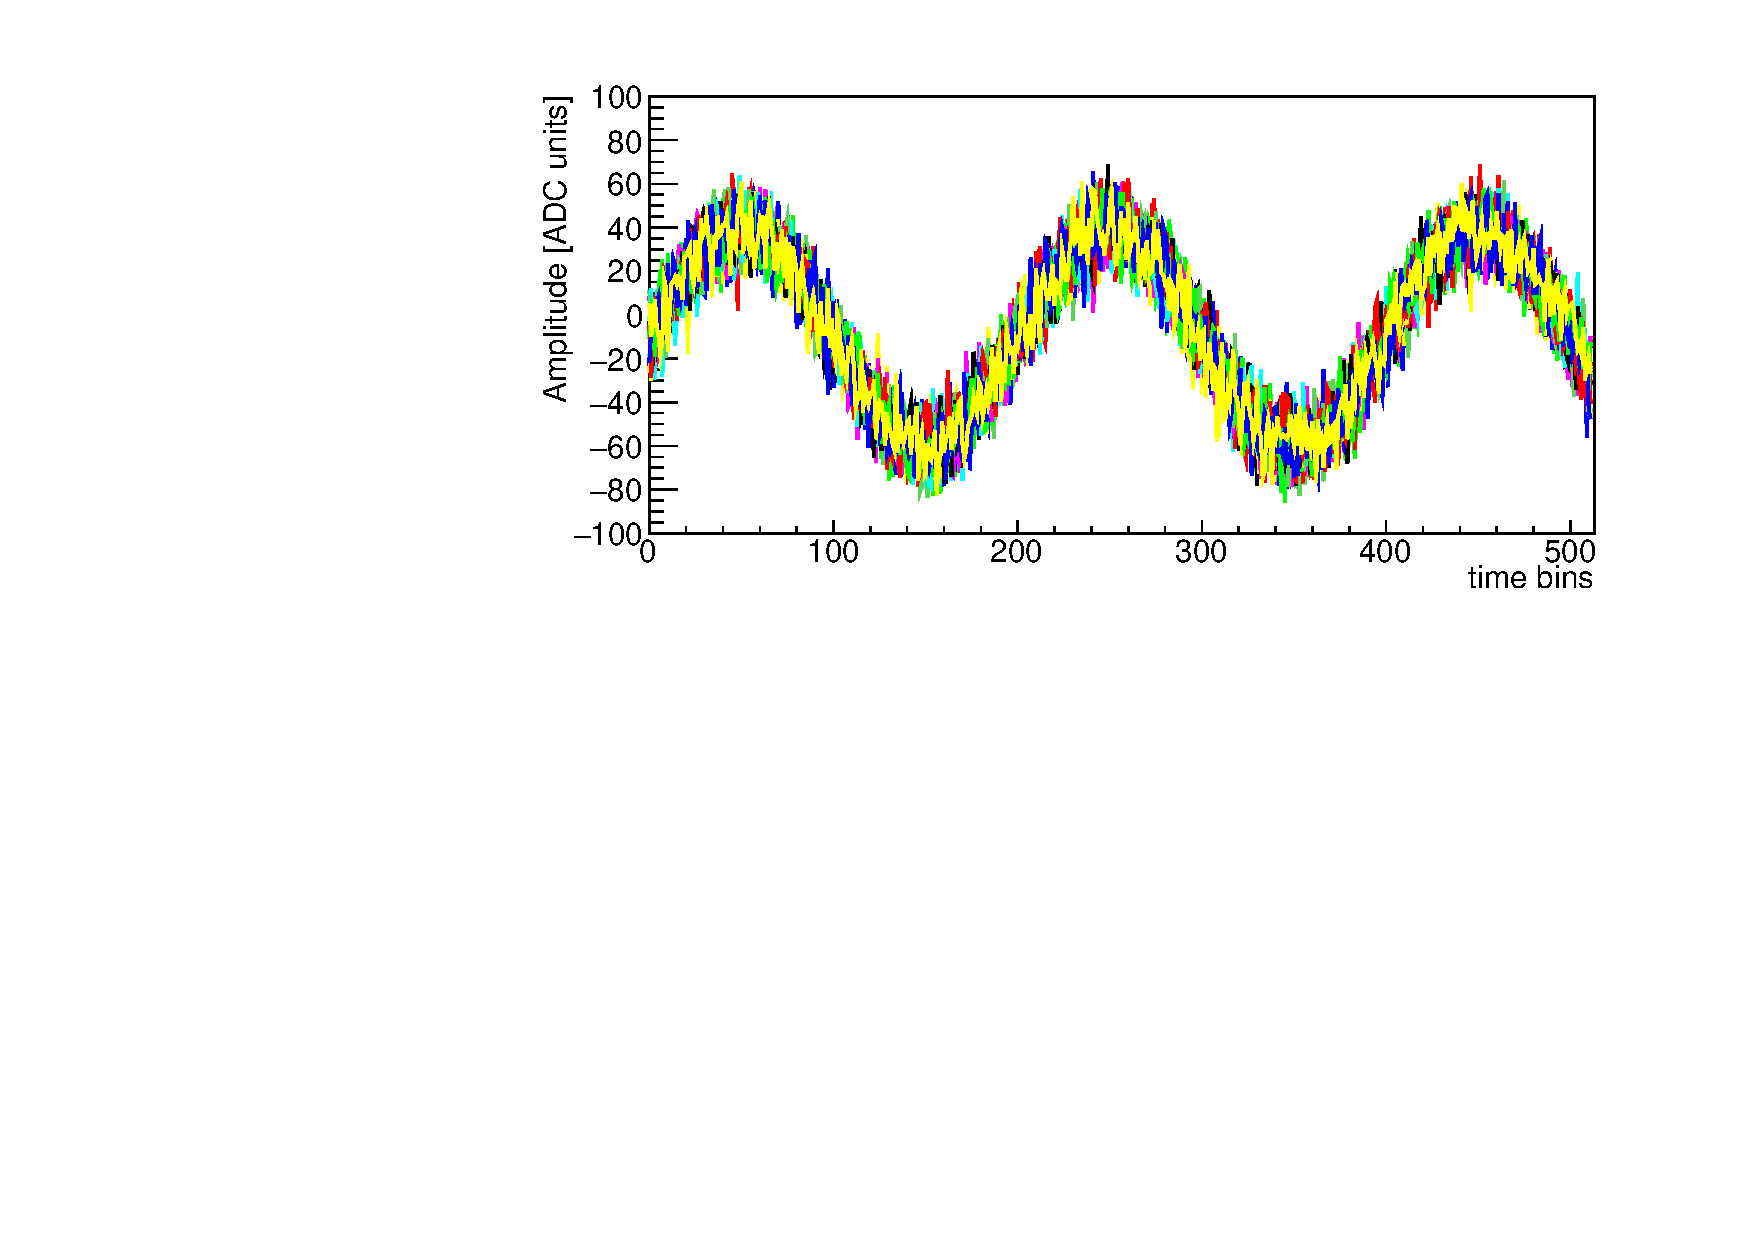
\includegraphics[width=0.48\textwidth]{images/sin.pdf} &
  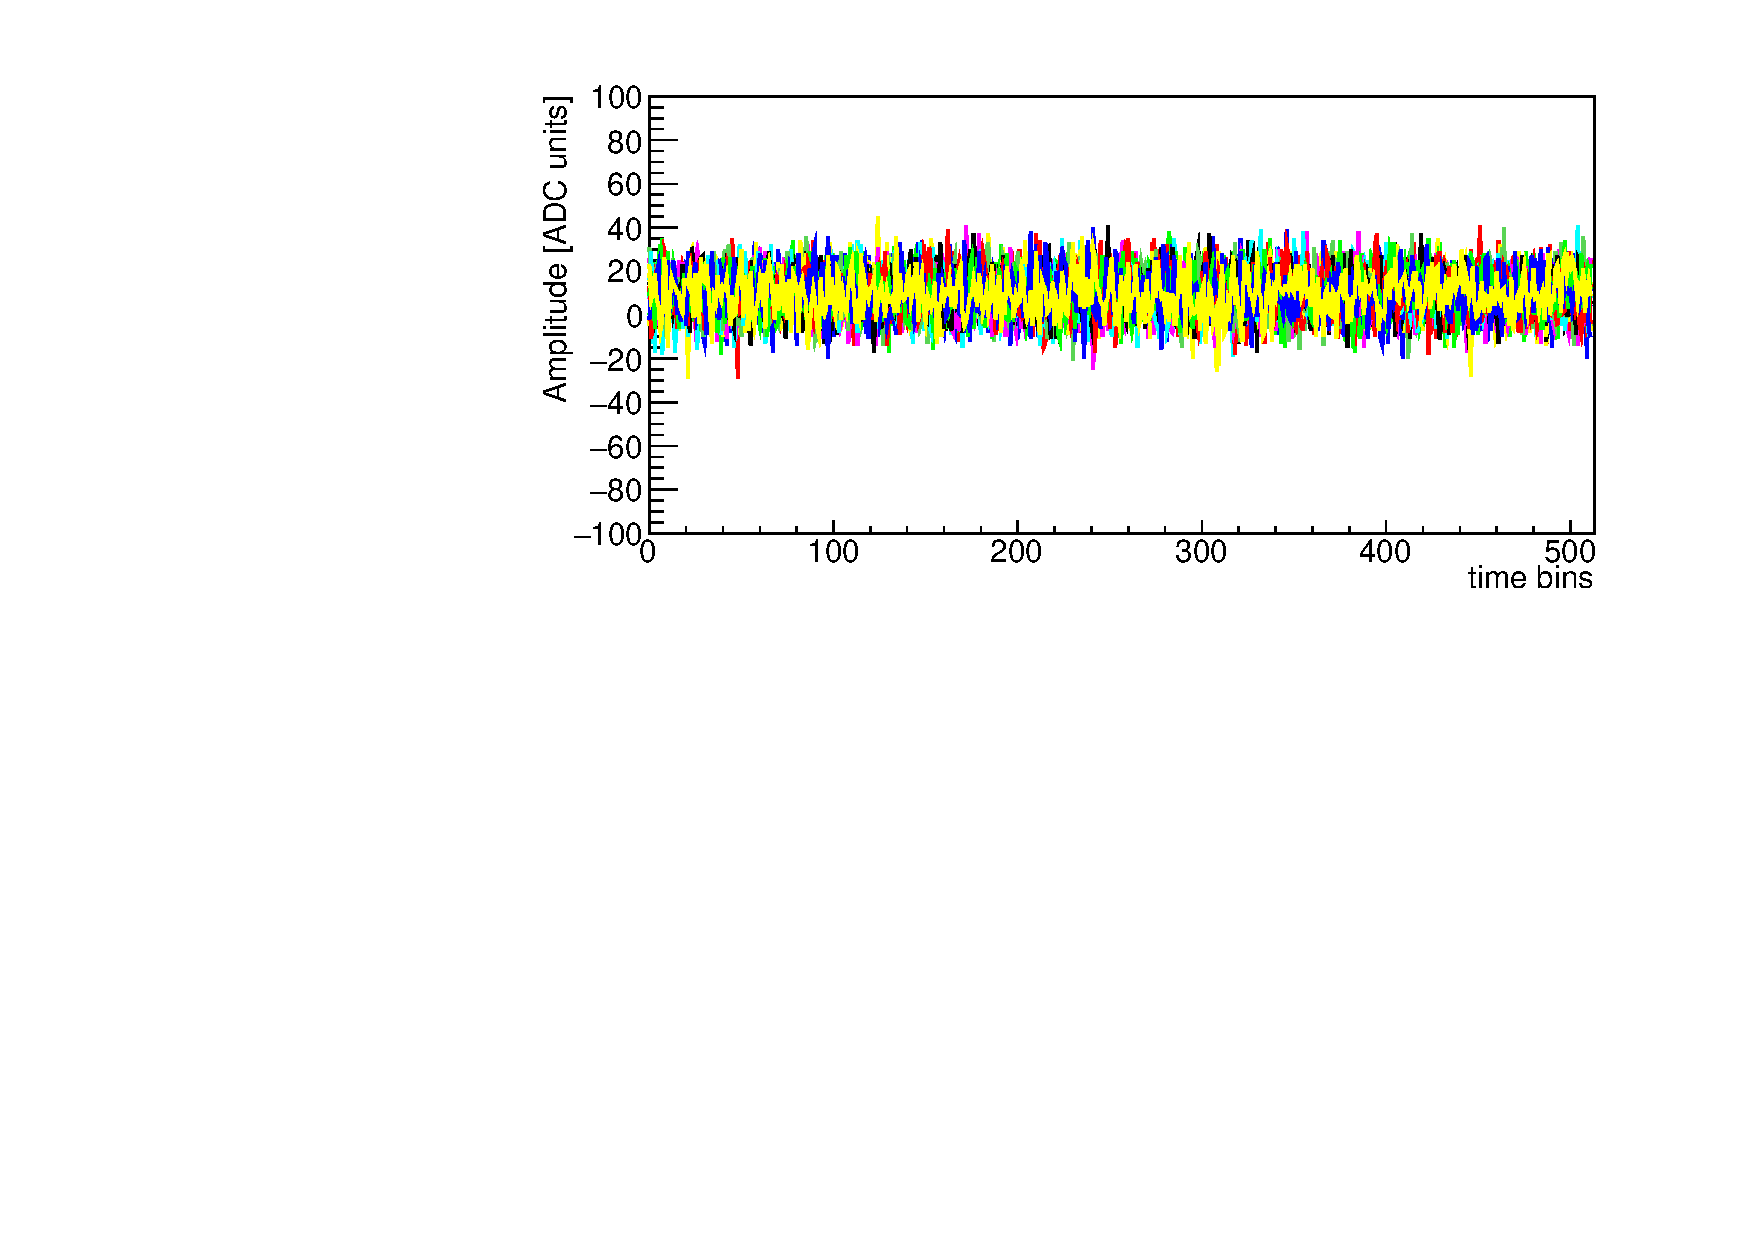
\includegraphics[width=0.48\textwidth]{images/clean.pdf} \\
  (a) & (b) \\
  
  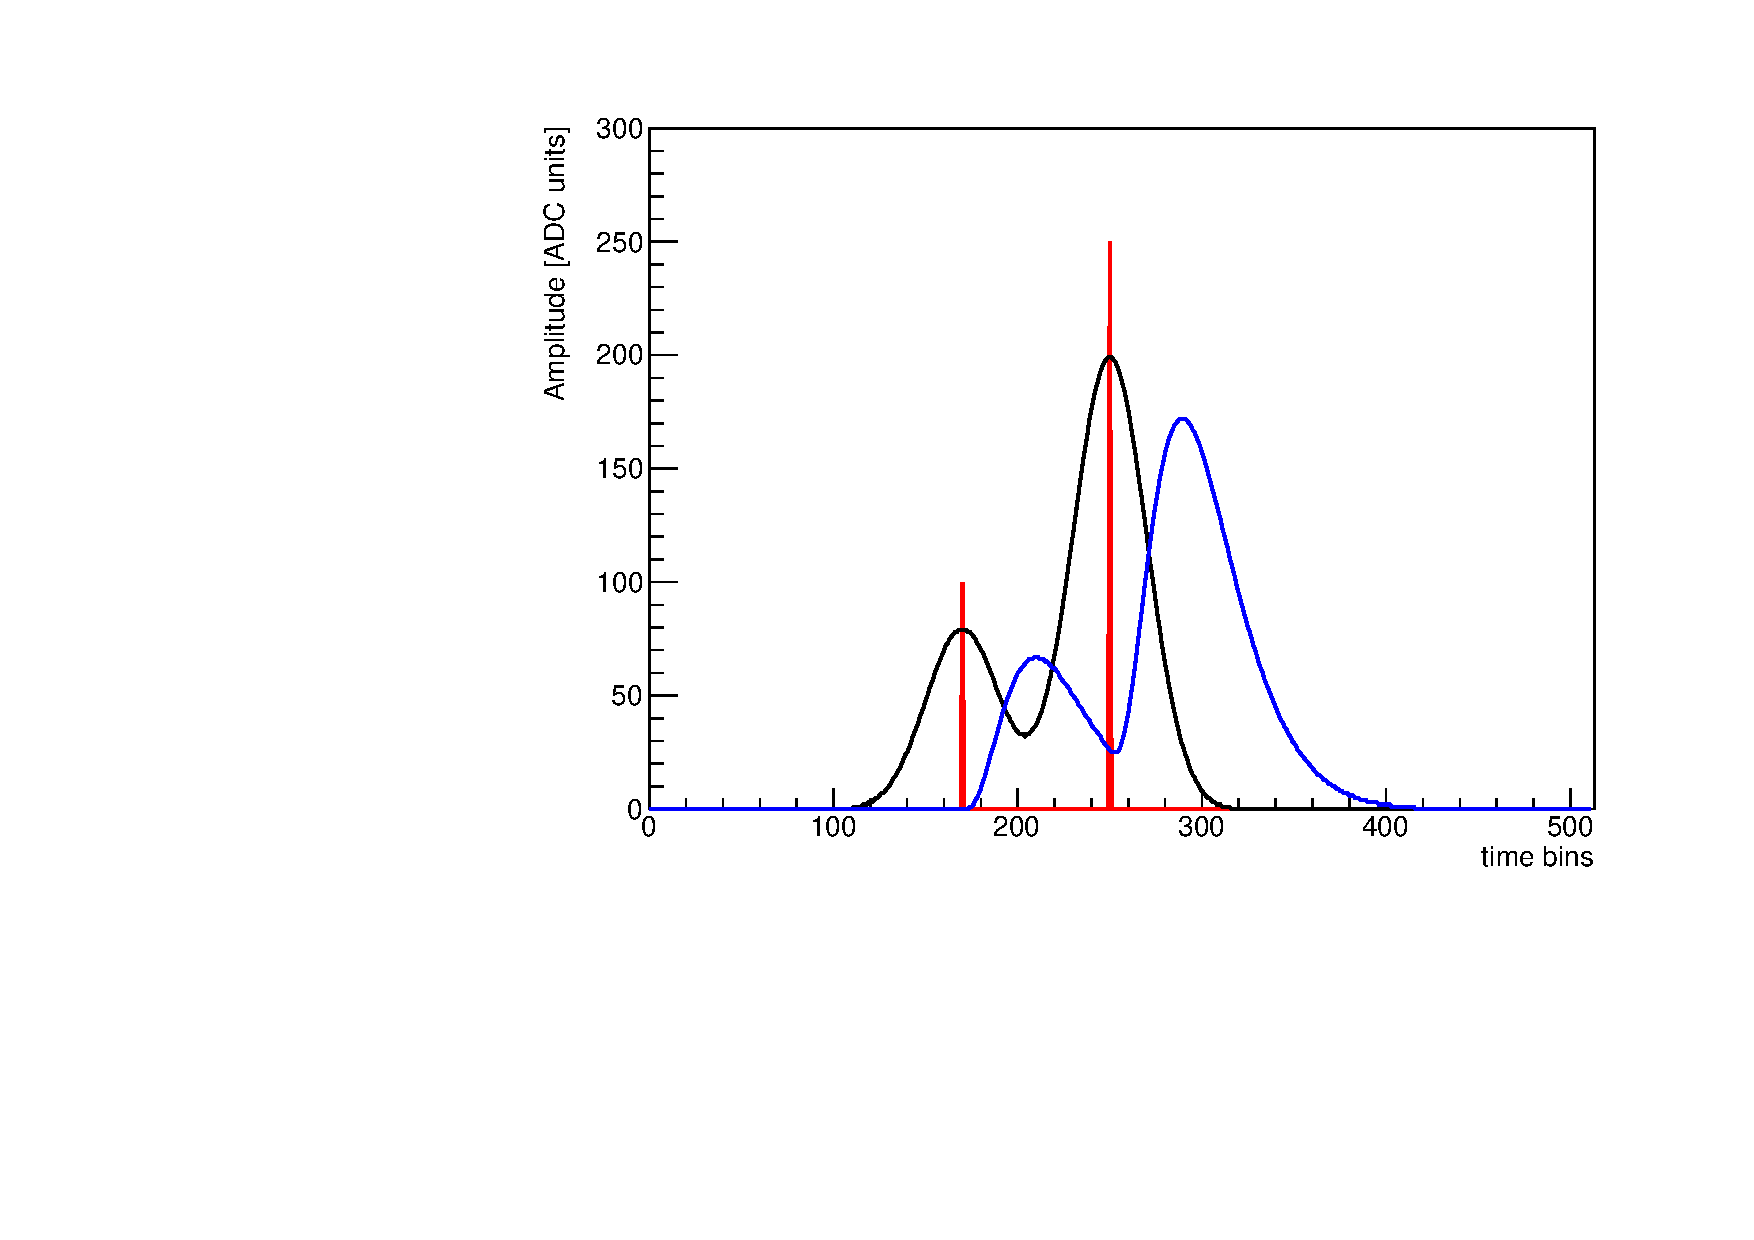
\includegraphics[width=0.46\textwidth]{images/shapingPlot.pdf} &
  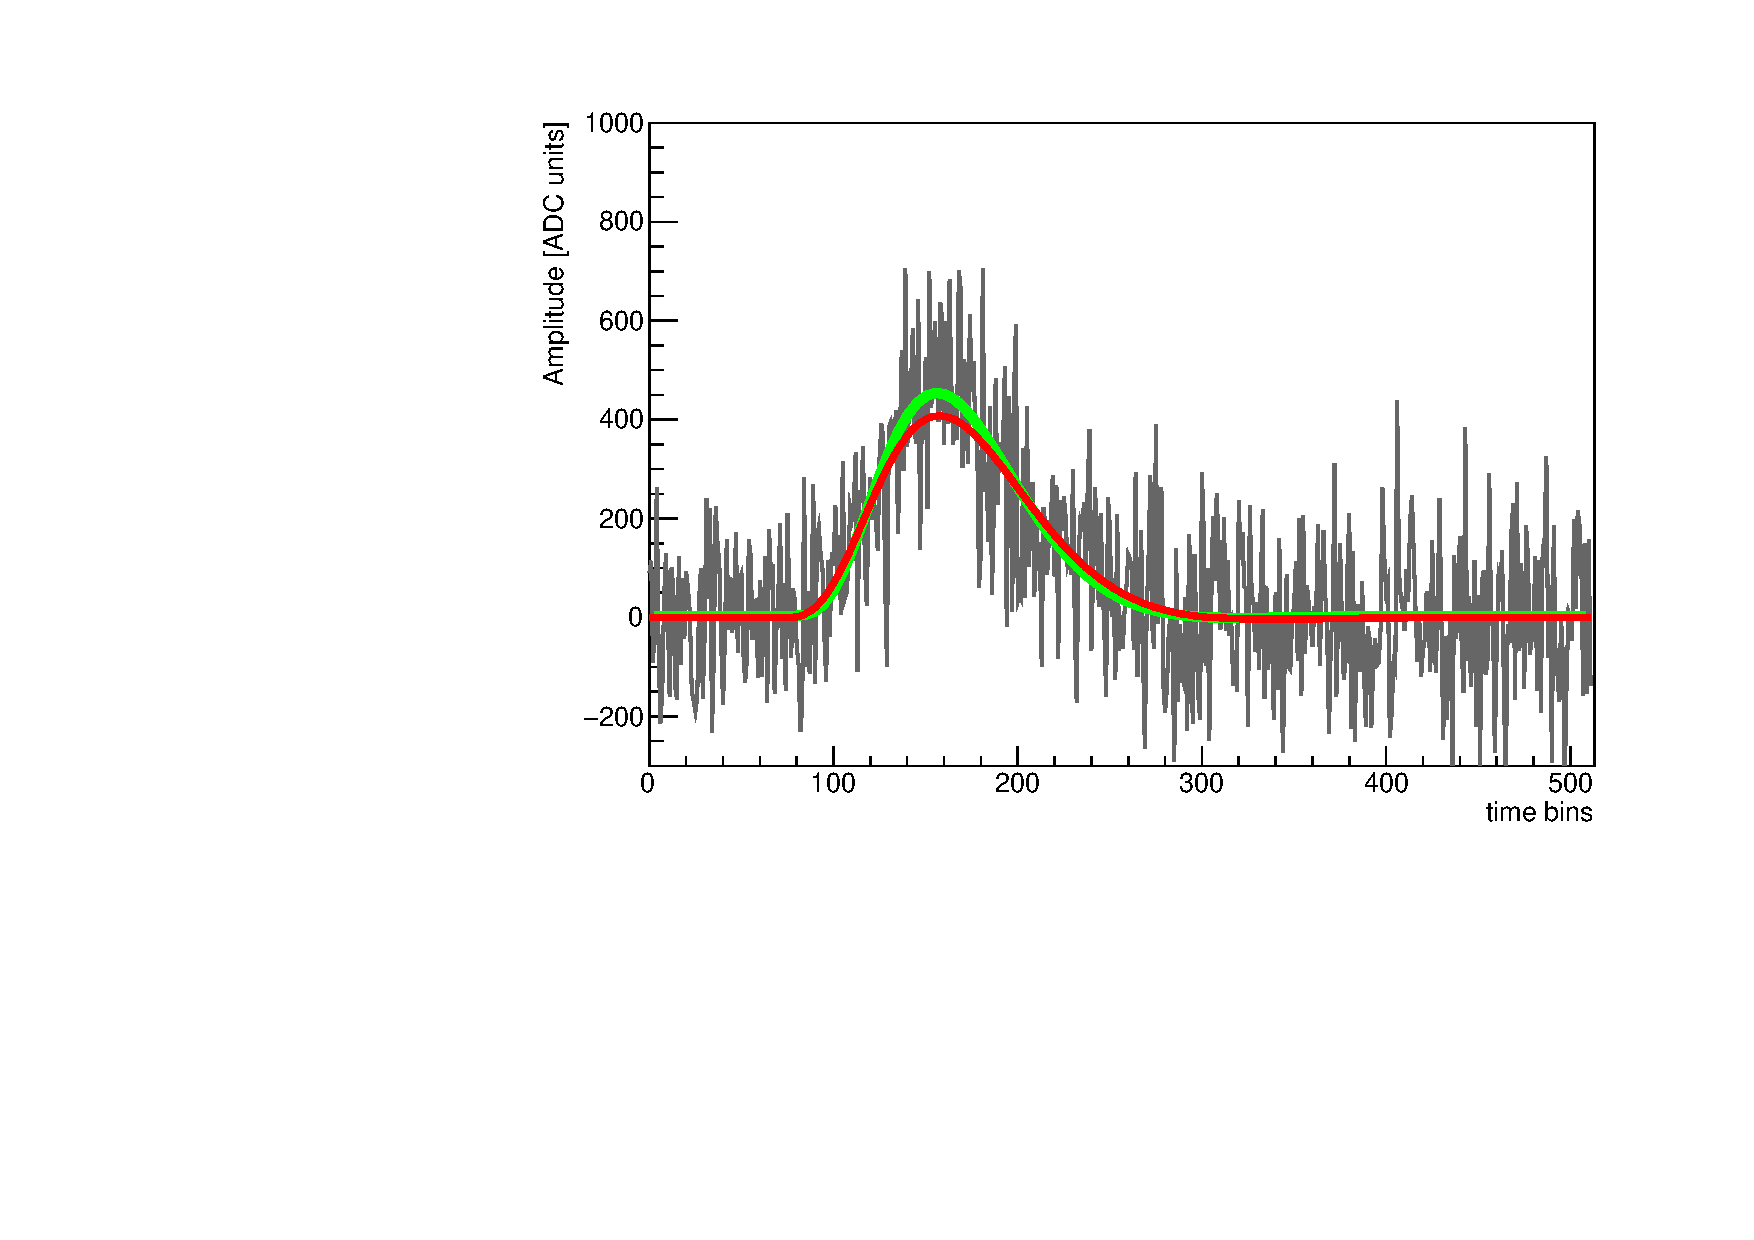
\includegraphics[width=0.48\textwidth]{images/fitComparison.pdf} \\
    (c) & (d) \\
  \end{tabular}
  }
	\caption{(a) An artificially-generated noise-\emph{raw signal event} with a common sinusoidal pattern. (b) The result after applying the \emph{common noise reduction} process to the event shown in (a), where only randomly added noise remains. (c) An idealized \emph{raw signal} composed of two point-like deposits (in red) is conditioned by the \emph{shaping} process using a Gaussian (in black) and an AGET electronics response (in blue) convolutions. (d) An artificially-generated noise-\emph{raw signal} (in black), together with the original pulse used to generate it (in red), and the recovered \emph{raw signal} after applying the \emph{fitting} process (in green).}\label{fig:rawlib}
\end{figure}

Apart from processes conditioning and treating a physical signal, the raw library includes processes, belonging to the external process type, that allow to importing into the framework the binary data generated by different electronics acquisition cards used in our field, such as AGET\,\cite{6154095} and AFTER\,\cite{Baron:2009sdx} chips, or DREAM\,\cite{Acker2020} electronics, among others.

\subsection{The geant4 library}\label{sc:geant4lib}

The geant4\footnote{We will use the lowercase version of the \emph{geant4} word when we refer to our own REST-for-Physics code implementation, while we will use the upper-case version, Geant4, to refer to the official CERN software package~\cite{Agostinelli:2002hh}. As a reminder, highlighted words provide a connection with the code objects, as \emph{geant4 event} being linked to the object \emph{TRestGeant4Event}.}  library\,\cite{REST_Geant4_Git} defines a \emph{geant4 event} type that registers the energy deposits, or hits, resulting from a Geant4 simulation. A Geant4 simulation performs the physics particle tracking including the interaction probability with the materials defined in a given detector geometry. The energy deposits are similar to those found at a \emph{detector hits event}, although the \emph{geant4 event} hits contain additional information,like the physical interaction process, the geometrical volume where the interaction took place or the remaining available kinetic energy of the particle that produced the energy deposit. The energy deposits are encapsulated into \emph{geant4 tracks} that describe properties common to a particular group of hits, such as the particle name producing the energy deposits, the position where the particle was originated, the track and parent ids, and in general, any relevant information directly extracted from the tracks produced by the Geant4 simulation package.

%Non-Geant4 dependency
It is important to mention that this library is not directly linked to the official Geant4 libraries. Its purpose is to store the event information generated by a Geant4 simulation, but once a simulation package has registered the information inside the \emph{geant4 event} data holder, the connection to Geant4 libraries is not required anymore. In a different perspective, a user would be able to access a Monte Carlo database of previously Geant4-generated files in REST format without the need to perform a system Geant4 installation.

%restG4 GDML
Inside the REST-for-Physics ecosystem we have developed an independent package, \emph{restG4}\,\cite{REST_restG4_Git}, which is a particular Geant4 code implementation taking advantage of the \emph{geant4 event} type and all the definitions available at the library to describe the simulation conditions. For example, the \emph{geant4 metadata} object defining the number of primaries to be generated, together with their energy and angular distributions, or the generator type, in order to determine how the primaries will be launched or initialized are defined here. There are many other options that allow the production of data sets in different experimental conditions and the definition of specific storage instructions. The library implements an additional metadata object, the \emph{geant4 physics list}, in which the particle physics processes to be considered inside the simulation package are registered and personalized. \emph{restG4} will register those metadata structures and the \emph{geant4 event} tree, together with a \emph{run} metadata object complying with the REST data format conventions so that the resulting data are ready to be further processed with this or other libraries available in REST. A simulation with \emph{restG4} requires as input the description of those 3 objects, the \emph{run}, the \emph{geant4 metadata} and the \emph{geant4 physics list}, through an \emph{rml} file, and a description of the geometry through a GDML\,\cite{Chytracek:2006be} file (see Figure\,\ref{fig:geant4lib}).



\begin{figure}[htb!]
  \centering
  \raisebox{-0.5\height}{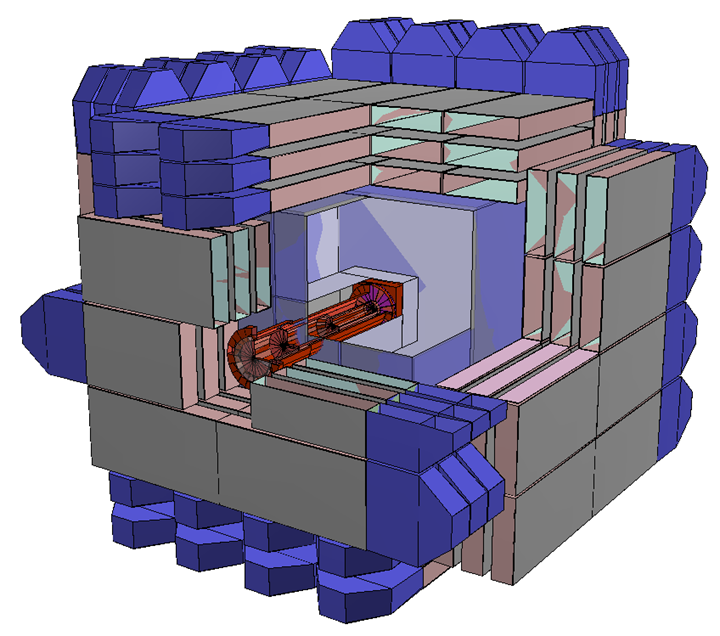
\includegraphics[width=0.4\textwidth]{images/BabyIAXO.png}\hspace{1 cm}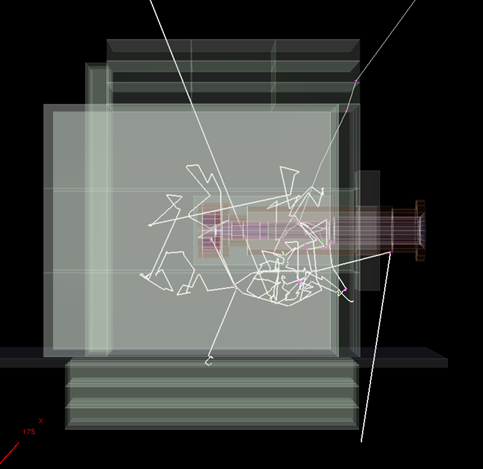
\includegraphics[width=0.35\textwidth]{images/neutron_event.png}}
	\caption{\emph{Left}, a visualization of the GDML geometry for the Baby-IAXO detector\,\cite{BabyIAXO:2020mzw}. \emph{Right}, a simulated cosmic neutron event at the same geometry visualized using the ROOT TEve viewer libraries.}\label{fig:geant4lib}
\end{figure}

%model
Once a first Monte Carlo data set has been generated using \emph{restG4} it can be processed using the existing routines in this library. These routines, or processes, can be used to extract the Monte Carlo truth at an early processing stage. One example is the \emph{blob analysis} process, aiming to extract the real electron track-ends at a $0\nu\beta\beta$ event: another is the \emph{neutron tagging} process allowing to produce elaborated observables to perform a detailed analysis of the interaction of neutrons with an active cosmic veto system. In general, there are available processes that introduce sophisticated physics models, the results of which will be written in the \emph{analysis tree} in the form of observables, to be accessed at a later stage of data treatment. The main idea, or philosophy, is that \emph{restG4} is simply used to generate a first data set, while the geant4 library will be used to introduce models that need to know about the nature of the particles or the interactions that produced the energy deposits inside the detector geometry. Once all the relevant information has been extracted and placed in the form of observables at the \emph{analysis tree} it can be migrated to other REST libraries (see section\,\ref{sc:connectorslib}) in order to include a detailed detector response, condition the data to mimic raw detector data, and perform the same data analysis processing applied to real experimental data.

\subsection{The track library}\label{sc:tracklib}

The track library\,\cite{REST_Track_Git} implements a \emph{track event} type that defines inheritance relations between a set of \emph{tracks} stored inside the event. A \emph{track} itself contains a group of hits (or cluster) that define a discrete energy distribution in a 3-dimensional coordinate space. In order to produce or initialize a first \emph{track event}, a process in the connectors library (section\,\ref{sc:connectorslib}) makes use of the \emph{detector hits event} as input to identify groups of hits, or energy deposits, that have a proximity relation, in order to create \emph{tracks}. It is important to remark that the \emph{track event} is an abstract object\footnote{Not to be confused with an abstract C++ class (it would have been highlighted otherwise). We want to emphasize that it is an object that does not have a strict or fixed scope.} that allows to define groups of hits, clusters, with an inheritance relation, i.e. we may develop \emph{track} levels by generating new daughter \emph{tracks} from the original ones. This could be exploited in different contexts: it could serve to describe random isolated clusters (or group of hits) in a single physical volume, or it could describe correlated \emph{tracks} at independent physical volumes by creating a new \emph{track} that incorporates all those mother tracks into one.

This library contains, on one hand, graph theory algorithms helping to identify and reconstruct physical tracks by finding the shortest path that interconnects energy deposits within a \emph{track}, and on the other, processes that allow to extract topological information from a \emph{track event}. Since graph theory algorithms are computationally expensive when dealing with a large number of nodes, a \emph{reduction} process can be used to decrease the effective number of \emph{hits}, so that Travelling Sales Problem (TSP) algorithms can be applied in an acceptable computation time. TSP methods help to find a reasonable solutions for the physical track identification, although further \emph{reconnection} algorithms may be needed to improve the result (see Figure\,\ref{fig:tracklib}). An important application of these algorithms is the identification of neutrinoless double beta decays, as it has been shown in the context of the PandaX-III experiment\,\cite{Galan:2019ake}.

\begin{figure}[htb!]
\centering
    \raisebox{-0.5\height}{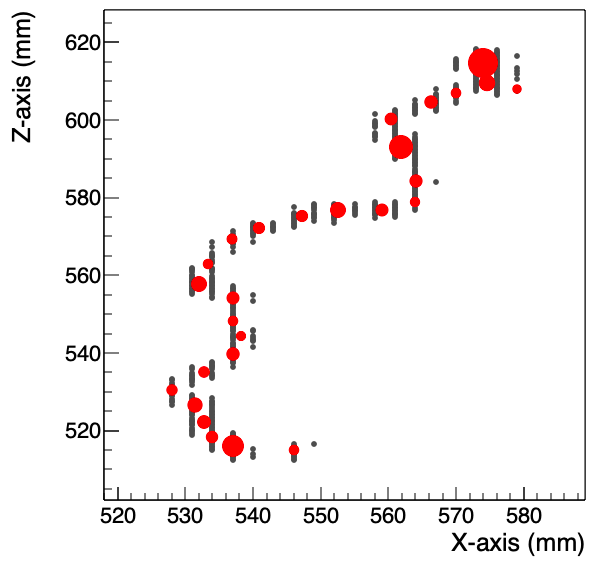
\includegraphics[width=0.33\textwidth]{images/TrackReduction.png}
    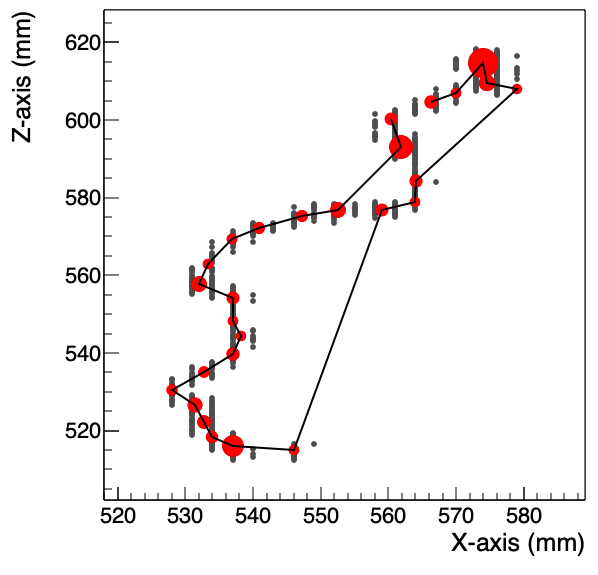
\includegraphics[width=0.33\textwidth]{images/TrackMinimized.png}
    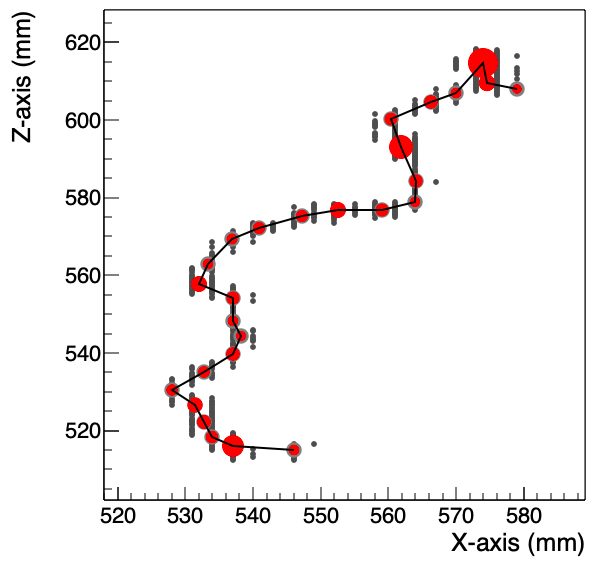
\includegraphics[width=0.33\textwidth]{images/TrackReconnected.png}}
    \caption{A \emph{track event} representation of a simulated $0\nu\beta\beta$ decay after the treatment with different \emph{track} processes used for physical track identification. \emph{Left}, an image of the hit reduction produced by the \emph{track reduction} process. The red circles represent the final position of reduced hits, whose size is weighted with their energy value. The small grey circles on the background represent the hits of the \emph{parent track} used as input. \emph{Middle}, a polyline is added to this representation to visualize the hits inter-connectivity after the \emph{track path minimization} process. If path minimization works on the whole, it produces at times obviously unphysical connections, as our example illustrates. \emph{Right}, the unphysical connections are corrected using a \emph{track reconnection} process. Figure extracted from reference\,\cite{Galan:2019ake}.}
    \label{fig:tracklib}
\end{figure}

\subsection{The connectors library}\label{sc:connectorslib}

The connectors library\,\cite{REST_Connectors_Git} contains class definitions that need to combine the features from classes residing in different REST-for-Physics libraries. This includes processes that transform the \emph{event} type from one library specific \emph{event} type into another library \emph{event} type, or it includes complex \emph{metadata} object descriptions that require combining specific metadata descriptions from different libraries. The main mission of this library is to keep inter-library dependencies isolated or encapsulated in a single entity. In this way the fundamental libraries described in previous sections will be operative in a stand-alone mode philosophy (see Figure\,\ref{fig:connectorslib}). The REST-for-Physics building system will compile only those connectors library classes related to libraries that were marked for compilation: in the extraordinary case that only a single library was marked, then the connectors library will not be compiled at all. This library differentiation helps the coherent development of independent libraries. Using this design any library may be enabled or disabled at will, avoiding unnecessary dependencies on dedicated systems.

\begin{figure}[htb!]
  \centering
  \raisebox{-0.5\height}{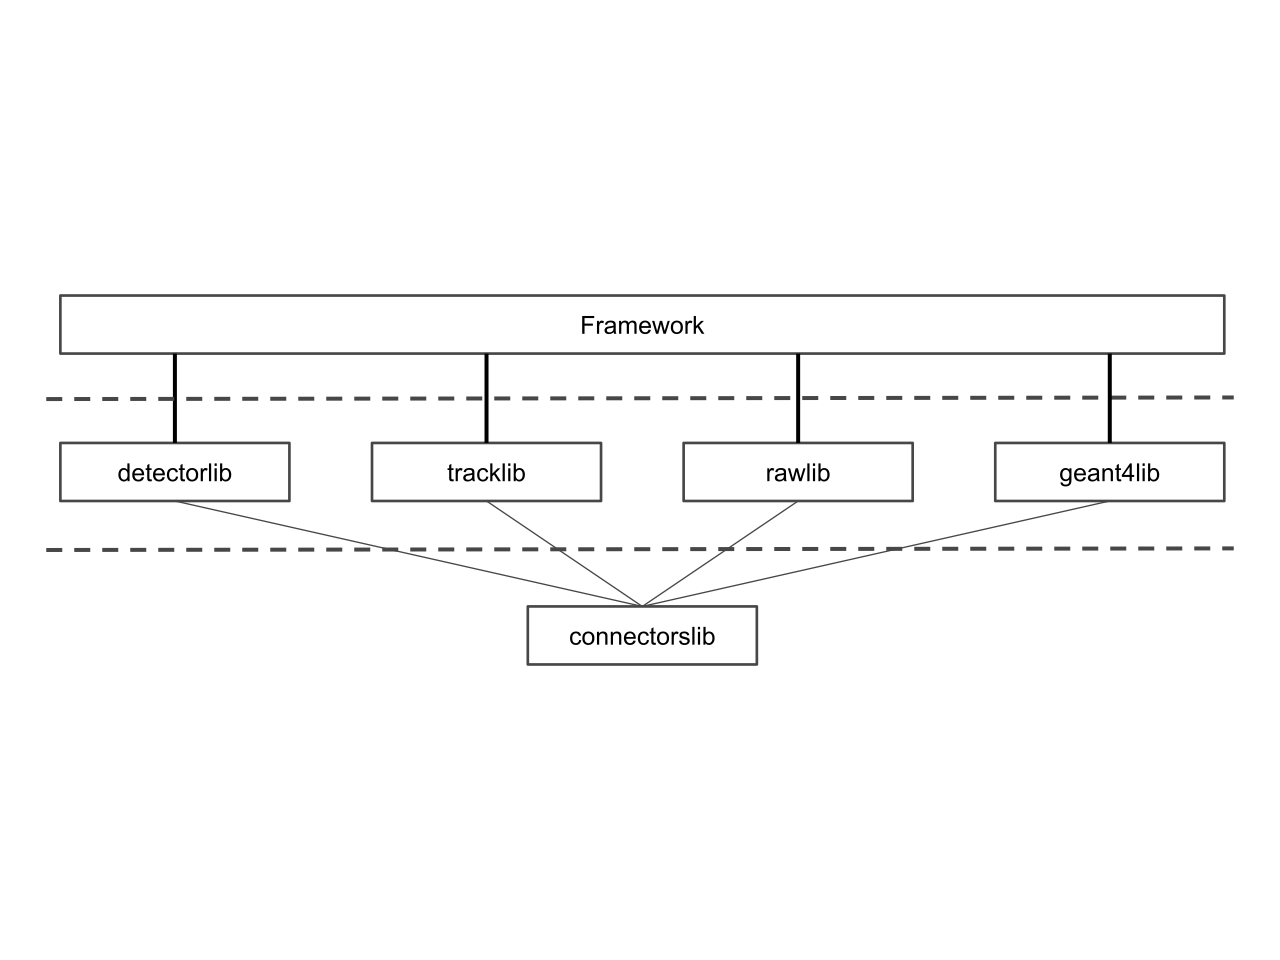
\includegraphics[trim=0 130 0 130, clip, width=0.75\linewidth]{images/connectorslib_new.png}}
	\caption{REST-for-Physics libraries hierarchy and connectivity to the framework. The connectors library depends on the other fundamental libraries, providing class definitions that help inter-library communication. On the other hand, fundamental libraries with a direct connection to the framework are capable to operate in a stand-alone mode, without any other REST-for-Physics libraries requirements.}\label{fig:connectorslib}
\end{figure}

Thus, the main functionality of this library is to allow moving from one fundamental library domain into another, transforming a \emph{raw signal event} into a \emph{detector signal event} by using data reduction techniques or grouping hits at a \emph{detector hits event} to produce a \emph{track event}. However, the connectors library must not be understood as a simple \emph{event} data type transformation, since the \emph{specific event} data usually requires sophisticated routines that include the detector physics involved for the event reconstruction, data reduction inside signal processing algorithms or graph theory for the clustering of hits. This library will play a crucial role to define how different library domains inter-connect.

%contains active routines

%not only i.e. hit clustering to transform detector hits into a track event, or raw signal to be transformed into a detector event. It also may contain other complex processes that require to use 2 libraries simultaneously.